\documentclass[conference]{IEEEtran}
\IEEEoverridecommandlockouts
% The preceding line is only needed to identify funding in the first footnote. If that is unneeded, please comment it out.
\usepackage{cite}
\usepackage{amsmath,amssymb,amsfonts}
\usepackage{algorithmic}
\usepackage{graphicx}
\usepackage{textcomp}
\usepackage{xcolor}
 \usepackage{multirow}

%---------------------------------
%By Ti
%%% Кодировки и шрифты %%%
\usepackage{cmap}						% Улучшенный поиск русских слов в полученном pdf-файле
\usepackage[utf8]{inputenc}				% Кодировка utf8
\usepackage[english, russian]{babel}    % Языки: русский, английский
\usepackage[T2A]{fontenc}				% Поддержка русских букв
\usepackage{pscyr}
\usepackage{booktabs}						% Красивые русские шрифты
%---------------------------------

\def\BibTeX{{\rm B\kern-.05em{\sc i\kern-.025em b}\kern-.08em
    T\kern-.1667em\lower.7ex\hbox{E}\kern-.125emX}}
\begin{document}

\title{Исследование эллиптической геометрической модели сердца для компьютерной многоканальной электроимпедансной кардиографии\\
%{\footnotesize \textsuperscript{*}Note: Sub-titles are not captured in Xplore and
%should not be used}
\thanks{The reported study was funded by RFBR according to the research project No 18-29-02042.}
}

\author{\IEEEauthorblockN{1\textsuperscript{st}  Alexey N. Tikhomirov}
\IEEEauthorblockA{\textit{Bauman Moscow State} \\
\textit{Technical University}\\
Moscow, Russia \\
tikhomirov.an@bmstu.ru}
\and
\IEEEauthorblockN{2\textsuperscript{nd} Andrey Briko}
\IEEEauthorblockA{\textit{Bauman Moscow State} \\
\textit{Technical University}\\
Moscow, Russia \\
briko@bmstu.ru}
\and
\IEEEauthorblockN{3\textsuperscript{rd} Nikolay Seleznev}
\IEEEauthorblockA{\textit{Bauman Moscow State} \\
\textit{Technical University}\\
Moscow, Russia \\
seleznev.nv@bk.ru}
\and
\IEEEauthorblockN{4\textsuperscript{th} Given Name Surname}
\IEEEauthorblockA{\textit{dept. name of organization (of Aff.)} \\
\textit{name of organization (of Aff.)}\\
City, Country \\
email address or ORCID}
\and
\IEEEauthorblockN{5\textsuperscript{th} Given Name Surname}
\IEEEauthorblockA{\textit{dept. name of organization (of Aff.)} \\
\textit{name of organization (of Aff.)}\\
City, Country \\
email address or ORCID}
\and
\IEEEauthorblockN{6\textsuperscript{th} Given Name Surname}
\IEEEauthorblockA{\textit{dept. name of organization (of Aff.)} \\
\textit{name of organization (of Aff.)}\\
City, Country \\
email address or ORCID}
}

\maketitle

\begin{abstract}
    абстракт

\end{abstract}

\begin{IEEEkeywords}
component, formatting, style, styling, insert
\end{IEEEkeywords}

\section{Introduction}

Ударный объем сердца, минутный объем и фракция выброса важные параметры при оценке состояния сердечно-сосудистой системы.
Эти параметры характеризуют гемодинамику деятельности сердца, являются гемодинамическими параметрами.

В клинической практике оценка гемодинамических параметров производится такими диагностическими методами, как КТ, МРТ, УЗИ.
Эти методы так же дают много дополнительной информации о сердце, однако мониторинг гемодинамических параметров сердца этими методами не возможен.
Частые периодические исследования дороги, а в случае с КТ являются вредной лучевой нагрузкой.

Термодилюционный метод с катетеризацией легочной артерии является золотым стандартом на сегодняшний день для оценки ударного выброса, однако  на практике применяется целый ряд инвазивных, малоинвазивных и неинвазивных методов (Kobe, Mishra 2019).

К минимально инвазивным методам можно отнести следующие методы.
Метод на основе делюции хлорида лития (Linton, Band 1993) используется в системе LiDCO.
К недостаткам системы можно отнести необходимость калибровки каждые 8 часов и при сильных изменениях гемодинамики сердца.
Также имеются противопоказания, связанные с реакцией организма на литий.
Системы PiCCO и FloTrac основаны на контурном анализе формы кривой давления, измеряемого инвазивно катетером, однако наличие регургитация клапанов, значительная аритмия и быстро меняющаяся температура влияют на точность измерений, основанных на таком методе.

Электроимпедансные методы исследования сердца и сердечно-сосудистой системы относятся к неинвазивным и недорогим.
Среди них выделяются трансторакальные методы, электроимпедансная томография и прекардиальная реокардиография.

Метод трансторакальной реокардиографии (ТРКГ) был разработан еще в середине XX века и в наше время с незначительными изменениями используется в таких аппаратах как CardioScreen(Medis), Рео-Спектр (Нейрософт).
Неинвазивные методы имеют меньше осложнений при использовании, но не лишены недостатков.
В основном метод ТРКГ используется для оценки изменения и наличия трендов при оценке гемодинамики, а не для определения абсолютных значений гемодинамических характеристик.

Метод электроимпедансной кардиографии находит свое применение в исследовании как легких, так и сердца.
Основным недостатком является низкое пространственное разрешение применительно к задаче оценки гемодинамики сердца.

Для расширения возможностей электроимпедансных методов исследования деятельности сердца, Стрелковым в 2002 году была предложена методика прекардиального картирования.

\section{Materials and methods}

\subsection{Методы прекардиальной реокардиографии}

Прекардиальная реокардиография объединяет несколько методов.
Во-первых, прекардиальное радиальное картирование.
Электродные системы располагаются вдоль границы проекции желудочков на поверхность грудной клетки перпендикулярно этой границе.
Во-вторых, продольно-поперечное картирование, при котором одна электродная система располагается на поверхности грудной клетки над сердцем вдоль анатомической оси сердца, а другая перпендикулярно ей.

Методы прекардиальной реокардиографии основаны на решении обратной задачи электроимпедансометрии.
Геометрическая модель строится на основе исходных данных, как правило, это данные КТ или МРТ.
%рассказать, что можно использовать не свежие данные
Сердце моделируется сферой, эллипсоидом или более сложной геометрией.
Сокращение сердца представляется изменением параметров модели, например радиуса сферы.
Экспериментально зарегистрированные изменения импеданса в ходе сокращения сердца пересчитываются в изменение параметров геометрической модели на основе решения обратной задачи, а затем оцениваются объемные характеристики.

Усложнение геометрической модели грудной клетки и сердца, формирует большее количество параметров, которые подробнее описывают сокращение сердца.
Однако это требует большего количество электродных систем для получения данных для решения обратной задачи электроимпедансометрии.

Таким образом, более сложная модель позволяет получать больше информации и требует большего количества электродных систем, более простая модель требует меньшего количества электродных систем, но ограничена в возможностях.
Необходимо искать компромисс между сложностью модели и получаемой информацией.

В задачах мониторинга гемодинамических характеристик зачастую важнее компактность и простота методики.
В данной работе сравниваются две геометрических модели однородного полупространства со включениями в виде сферы и эллипсоида.
Обе модели рассматриваются для метода прекардиального продольно-поперечного картирования сердца.

\subsection{Модель сферы и эллипсоида}

%\begin{figure}[tbph]
%    \centering
%    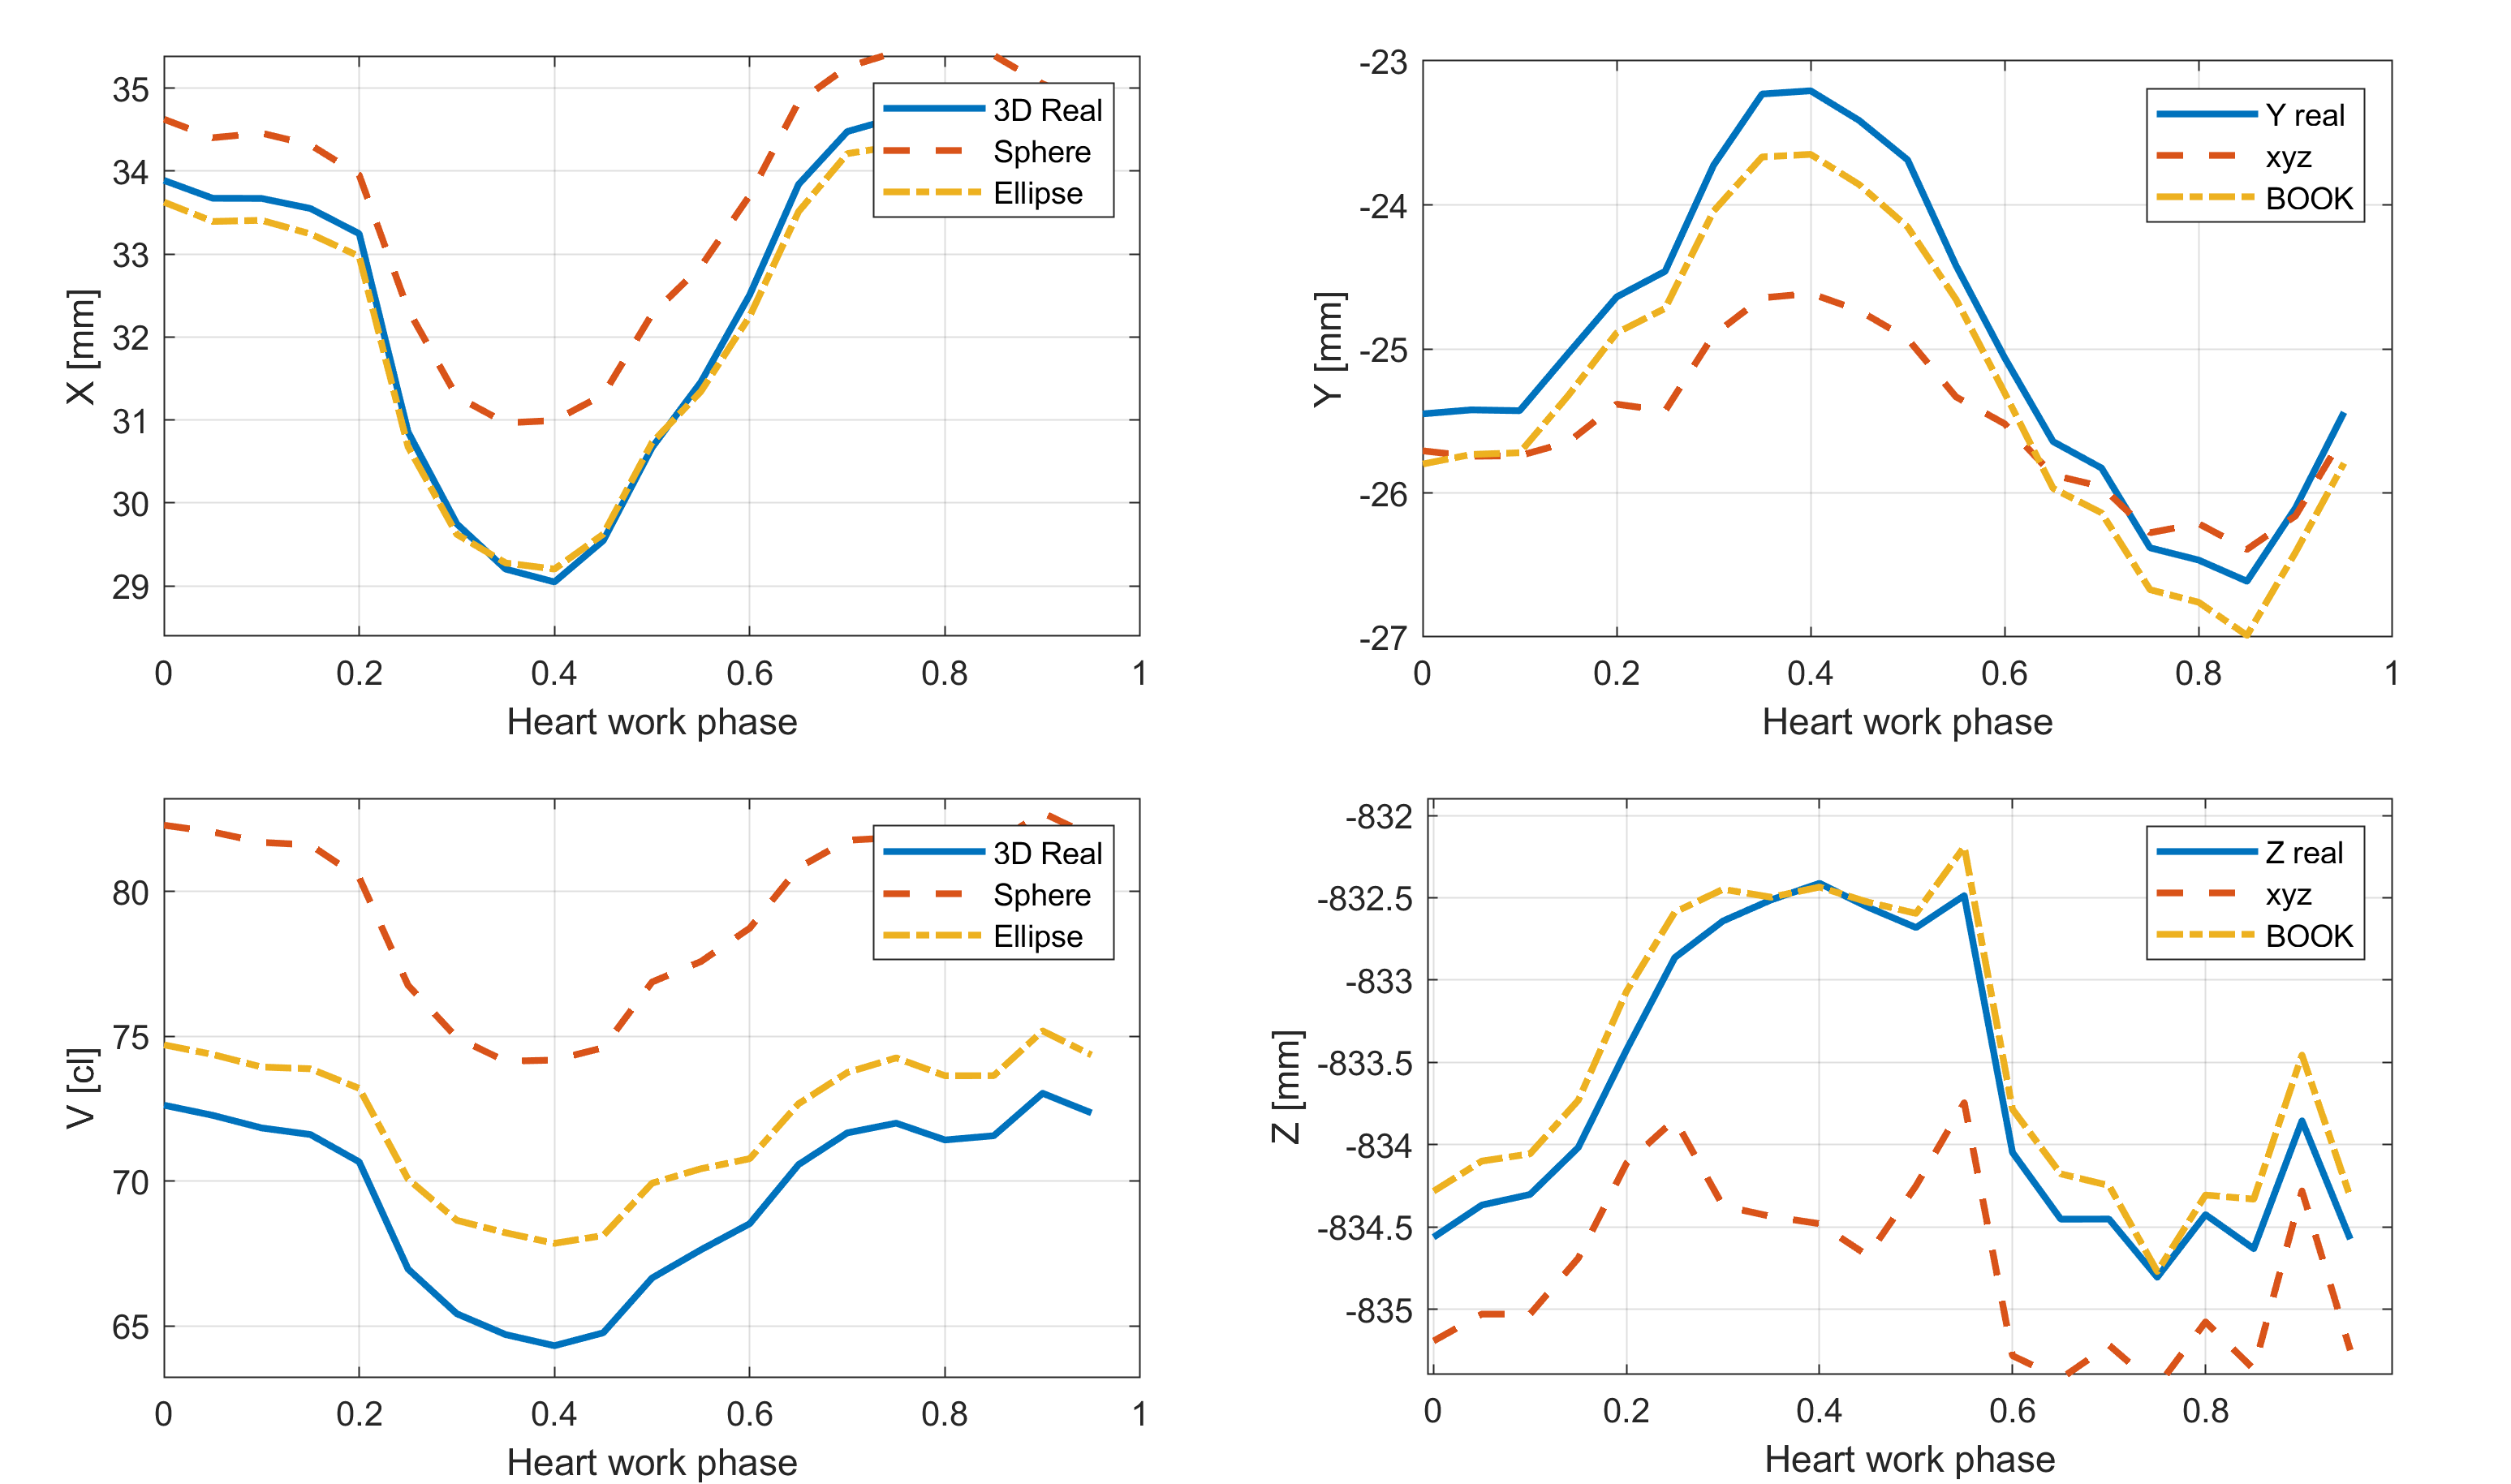
\includegraphics[width=\linewidth]{fig/1_4}
%    \caption{}
%    \label{fig:14}
%\end{figure}

При моделировании кровь в сердце часто представляется в виде сферы в задачах электроимпедансометрии, как в методах прекардиального картирования,
%[наши статьи]
так и в методах электроимпедансной томографии сердца.
%[статьи по томографии]
Данная модель достаточно проста.
По данным томографии определяются параметры сферы - радиус и координаты центра.
Сокращение сердца соответствует изменению радиуса сферы и смещению её центра.

Использование модели эллипсоида позволяет лучше аппроксимировать кровь в сердце перед началом систолы желудочков.
% статьи по эллипсу
Однако, количество параметров модели увеличивается - три полуоси эллипсоида, координаты центра и поворот эллипсоида в пространстве.
Сокращение сердца соответсвует изменению полуосей эллипсоида и смещению его центра.
Также возможен поворот в пространстве модели сердца при сокращении.

Геометрические параметры моделей были получены по данным компьютерной томограммы здорового добровольца.
Исследование мультиспиральной компьютерной томографии проводилось в Городской Клинической Больнице №1 им. Н.И. Пирогова города Москвы на аппарате Toshiba
Aquilion PRIME 160 и под патронажем сотрудников как клиники.
%, так и медицинского центра МГТУ им. Н.Э. Баумана.

Исследование проводилось с введением йодосодержащего контрастного вещества оптирей 350 мг,
%по 90 мл при исследовании на вдохе и 90 мл при исследовании на выдохе,
50мл со скоростью 3,5 мл/сек и 40 мл со скоростью 3 мл/сек.

Исследование проводилось на свободном выдохе.
В результате реконструкции данных исследований были получены наборы срезов
с временным разрешением 20 серий на один кардиоцикл, что составляет порядка 35-50 мс
в зависимости от ЧСС.
Расстояние между аксиальными срезами составило 2,5 мм.
По наборам срезов производилась реконструкция 3D модели крови в сердце.

\subsection{Аппроксимация сферой и эллипсоидом}
Параметры сферы и эллипсоида получались аппроксимацией 3D моделей крови сердца.

Сфера аппроксимировалась по критерию наименьшего квадратичного отклонения границ сферы и реальной 3D геометрии.
Критерий аппроксимации \ref{eq:sphere_criteria},
где $ p_i$ - конечное множество точек поверхности 3D модели сердца,
$dist(p_i,Z(f))$ - расстояние от точки $ p_i$ до поверхности сферы $Z(f)$.
\begin{equation}
    \sum_{i=1}^{q}dist(p_i,Z(f))^2 \rightarrow min
    \label{eq:sphere_criteria}
\end{equation}

Эллипсоид получался по критерию, описанному в .
%todo добавить ссылку на статью BOOK
Особенностью метода является то, что авторы рассматривают расстояние от точки до эллипсоида
$dist(p_i,Z(f))$, как разность между расстоянием от центра эллипсоида до точки и расстоянием от центра
эллипсоида до точки на его границе, лежащей на луче, выходящем их центра и проходящем через заданную точку.
Затем оценивается погрешность этого допущения в зависимости от соотношения полуосей эллипсоида и вносится корректировка.
Итоговым критерием оптимизации также является метод наименьших квадратов (2).

Анализ результатов и визуализации аппроксимации показал, что внутренние перегородки сердца, такие как межжелудочковая перегородка,
%todo ссылка на рисунок модели серца
предсердно-желудочковая перегородка(Рис.~\ref{fig:wall}), формируют точки, которые искажают результаты аппроксимации,
вызывая увеличение среднего отклонения поверхности аппроксимирующего эллипса или сферы от внешней границы 3D модели крови.

\begin{figure}[tbph]
    \centering
    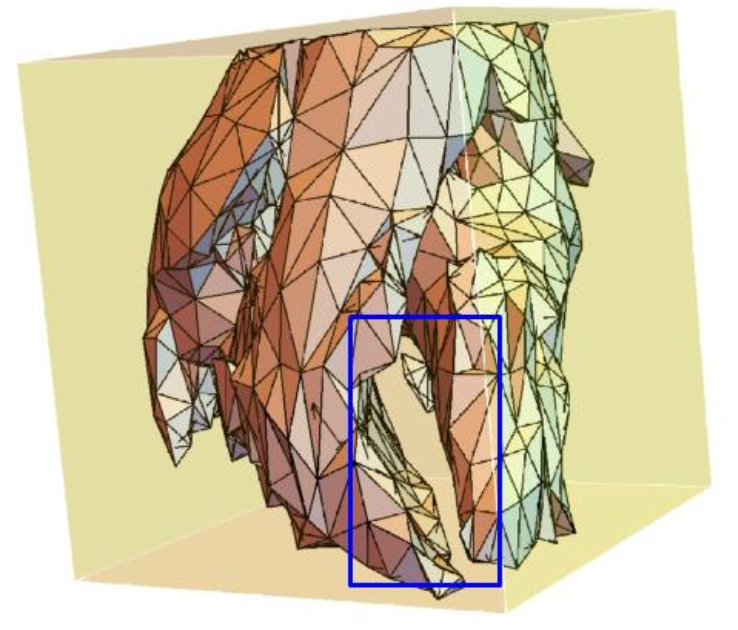
\includegraphics[width=0.8\linewidth]{fig/wall}
    \caption{3D модель крови в сердце (межжелудочковая перегородка выделена синим
    цветом)}
    \label{fig:wall}
\end{figure}

Для устранения этой проблемы было решено в исходных 3D моделях сердца заполнить перегородки и внутренние пустоты.
Для этого 3D модель раскладывалась на 2D изображения, полученные сечением плоскостями параллельными осям X и Y (Рис.~\ref{fig:algo}).
%--------------------------------------------------------
\begin{figure}[tbph]
    \centering
    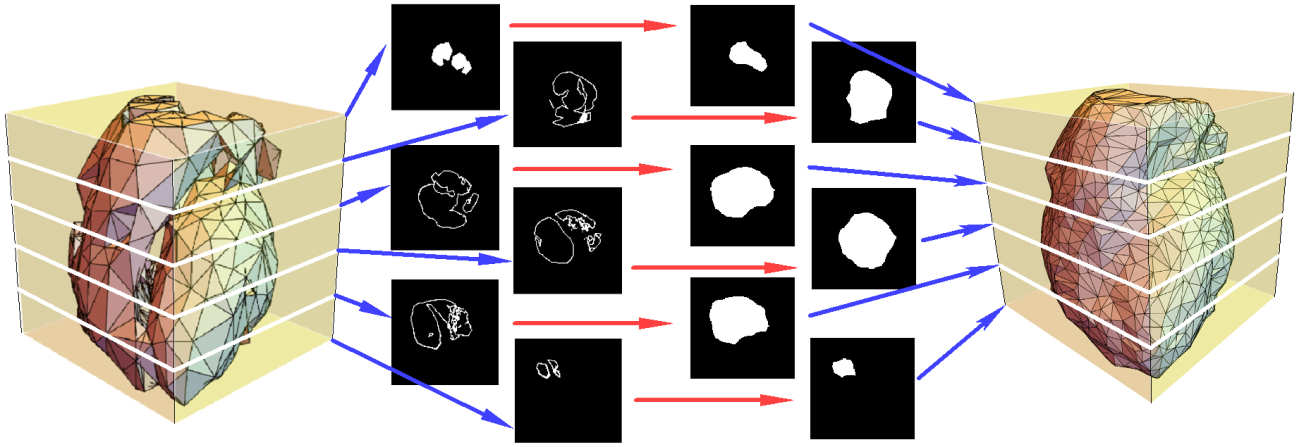
\includegraphics[width=\linewidth]{fig/algo}
    \caption{Алгоритм заполнения перегородок сердца в 3D модели крови сердца (слева –
    исходная 3D модель, справа – 3D модель после заполнения перегородок)}
    \label{fig:algo}
\end{figure}
%---------------------------------------------------------
Затем производился обход по касательной, контура 2D изображения окружностью радиусом
20 мм (красная окружность), в результате набор полученных срезов с заполненной перегородкой собирался в 3D изображение сердца (Рис.~\ref{fig:algo2}).

\begin{figure}[tbph]
    \centering
    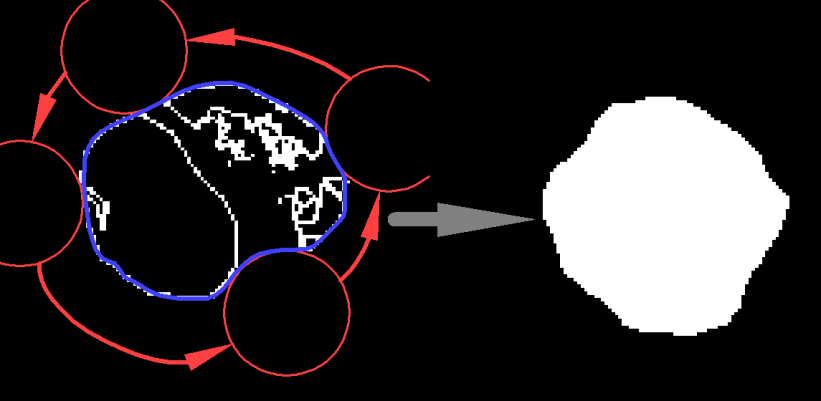
\includegraphics[width=\linewidth]{fig/algo2}
    \caption{Обход контура 2D изображения окружностью для заполнения перегородок
    сердца в 3D моделях крови сердца (слева – белый контур до заполнения перегородок,
        справа – после заполнения перегородок)}
    \label{fig:algo2}
\end{figure}

\section{Моделирование}
\section{Параметры электроимпедансного моделирования}
Для анализа полученных геометрических моделей проводилось электроимпедансное моделирование в среде конечно-элементного анализа Comsol Multiphisics.
Расположение электродных систем при моделировании соответствовало расположению электродных систем при продольно-поперечном картировании. Расстояние между токовыми электродами варьировалось от 80 до 240 мм, а отношение расстояния между токовыми электродами к расстоянию между потенциальными составляло 2 к 1.

Значения удельных сопротивлений включения и однородного полупространства представлены в таблице \ref{tab:table}.

\begin{table}[htbp]
    \caption{RESISTIVITY VALUES AT 100 KHZ USED IN THE MODEL STUDY}
    \begin{center}
        \begin{tabular}{|l|c|c|}
            \hline
            \multirow{2}{*}{\textbf{Tissue}}              &     \textbf{Resistivity values,}      &    \textbf{Resistivity value in}  \\
            &    \textbf{ Omh*m}     &   \textbf{ simulation, Omh*m }\\
            \hline
            Blood (Hct=50)           & 1.35 [21]           & 1.35      \\
            \hline
            Myocardium               & 4.6 [20]       & \multirow{7}{*}{4.2}\\
            \cline{1-2}
            \multirow{2}{*}{Muscles} & 2.7 [20]          &     \\
            \cline{2-2}
            & 1.5 – 25 [19]           &   \\
            \cline{1-2}
            Lung (deflated)          & 3.68 [20]     &         \\
            \cline{1-2}
            Lung                     & 1.6 – 10 [1]       &    \\
            \cline{1-2}
            Human thorax & \multirow{2}{*}{4.63 [19]}  &   \\
            (average)   & &   \\
            \hline
        \end{tabular}
        \label{tab:table}
    \end{center}
\end{table}
%todo поправить список литературы в таблице

Усреднение удельных сопротивлений легочной, мышечной ткани и миокарда возможно, так как рассматриваются измерения в фазу спокойного выдоха, а удельное сопротивление легочной ткани на выдохе приближается к удельному сопротивлению мышечной ткани.

\subsection{Сравние 3D моели со сферой и эллипсоидом}

По нескольким параметрам сравнивались сами модели и результаты моделирования реальной 3D геометрии крови в сердце, сферы и эллипсоида.
Во-первых, производилось сравнение изменения объема крови в сердце, то есть объема реальной 3D модели, с объемами аппроксимирующих сферы и эллипса. Оценка объемов производилась для каждого из 20 моментов времени, на которые разбивался кардиоцикл.
Во-вторых, рассматривалось движение объема крови в сердце в целом, то есть движение центра масс реальной 3D модели и аппроксимирующих её фигур.
В- третьих, сравнивались зависимости изменения импеданса в ходе сердечного цикла для различных расположений и размеров электродных систем.

\begin{figure}[htbp]
%    \centerline{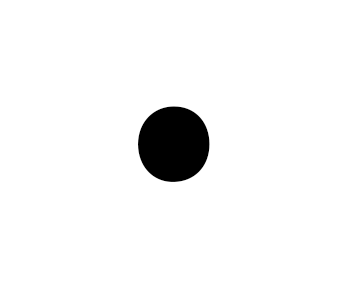
\includegraphics{fig/fig1.png}}
    \centering{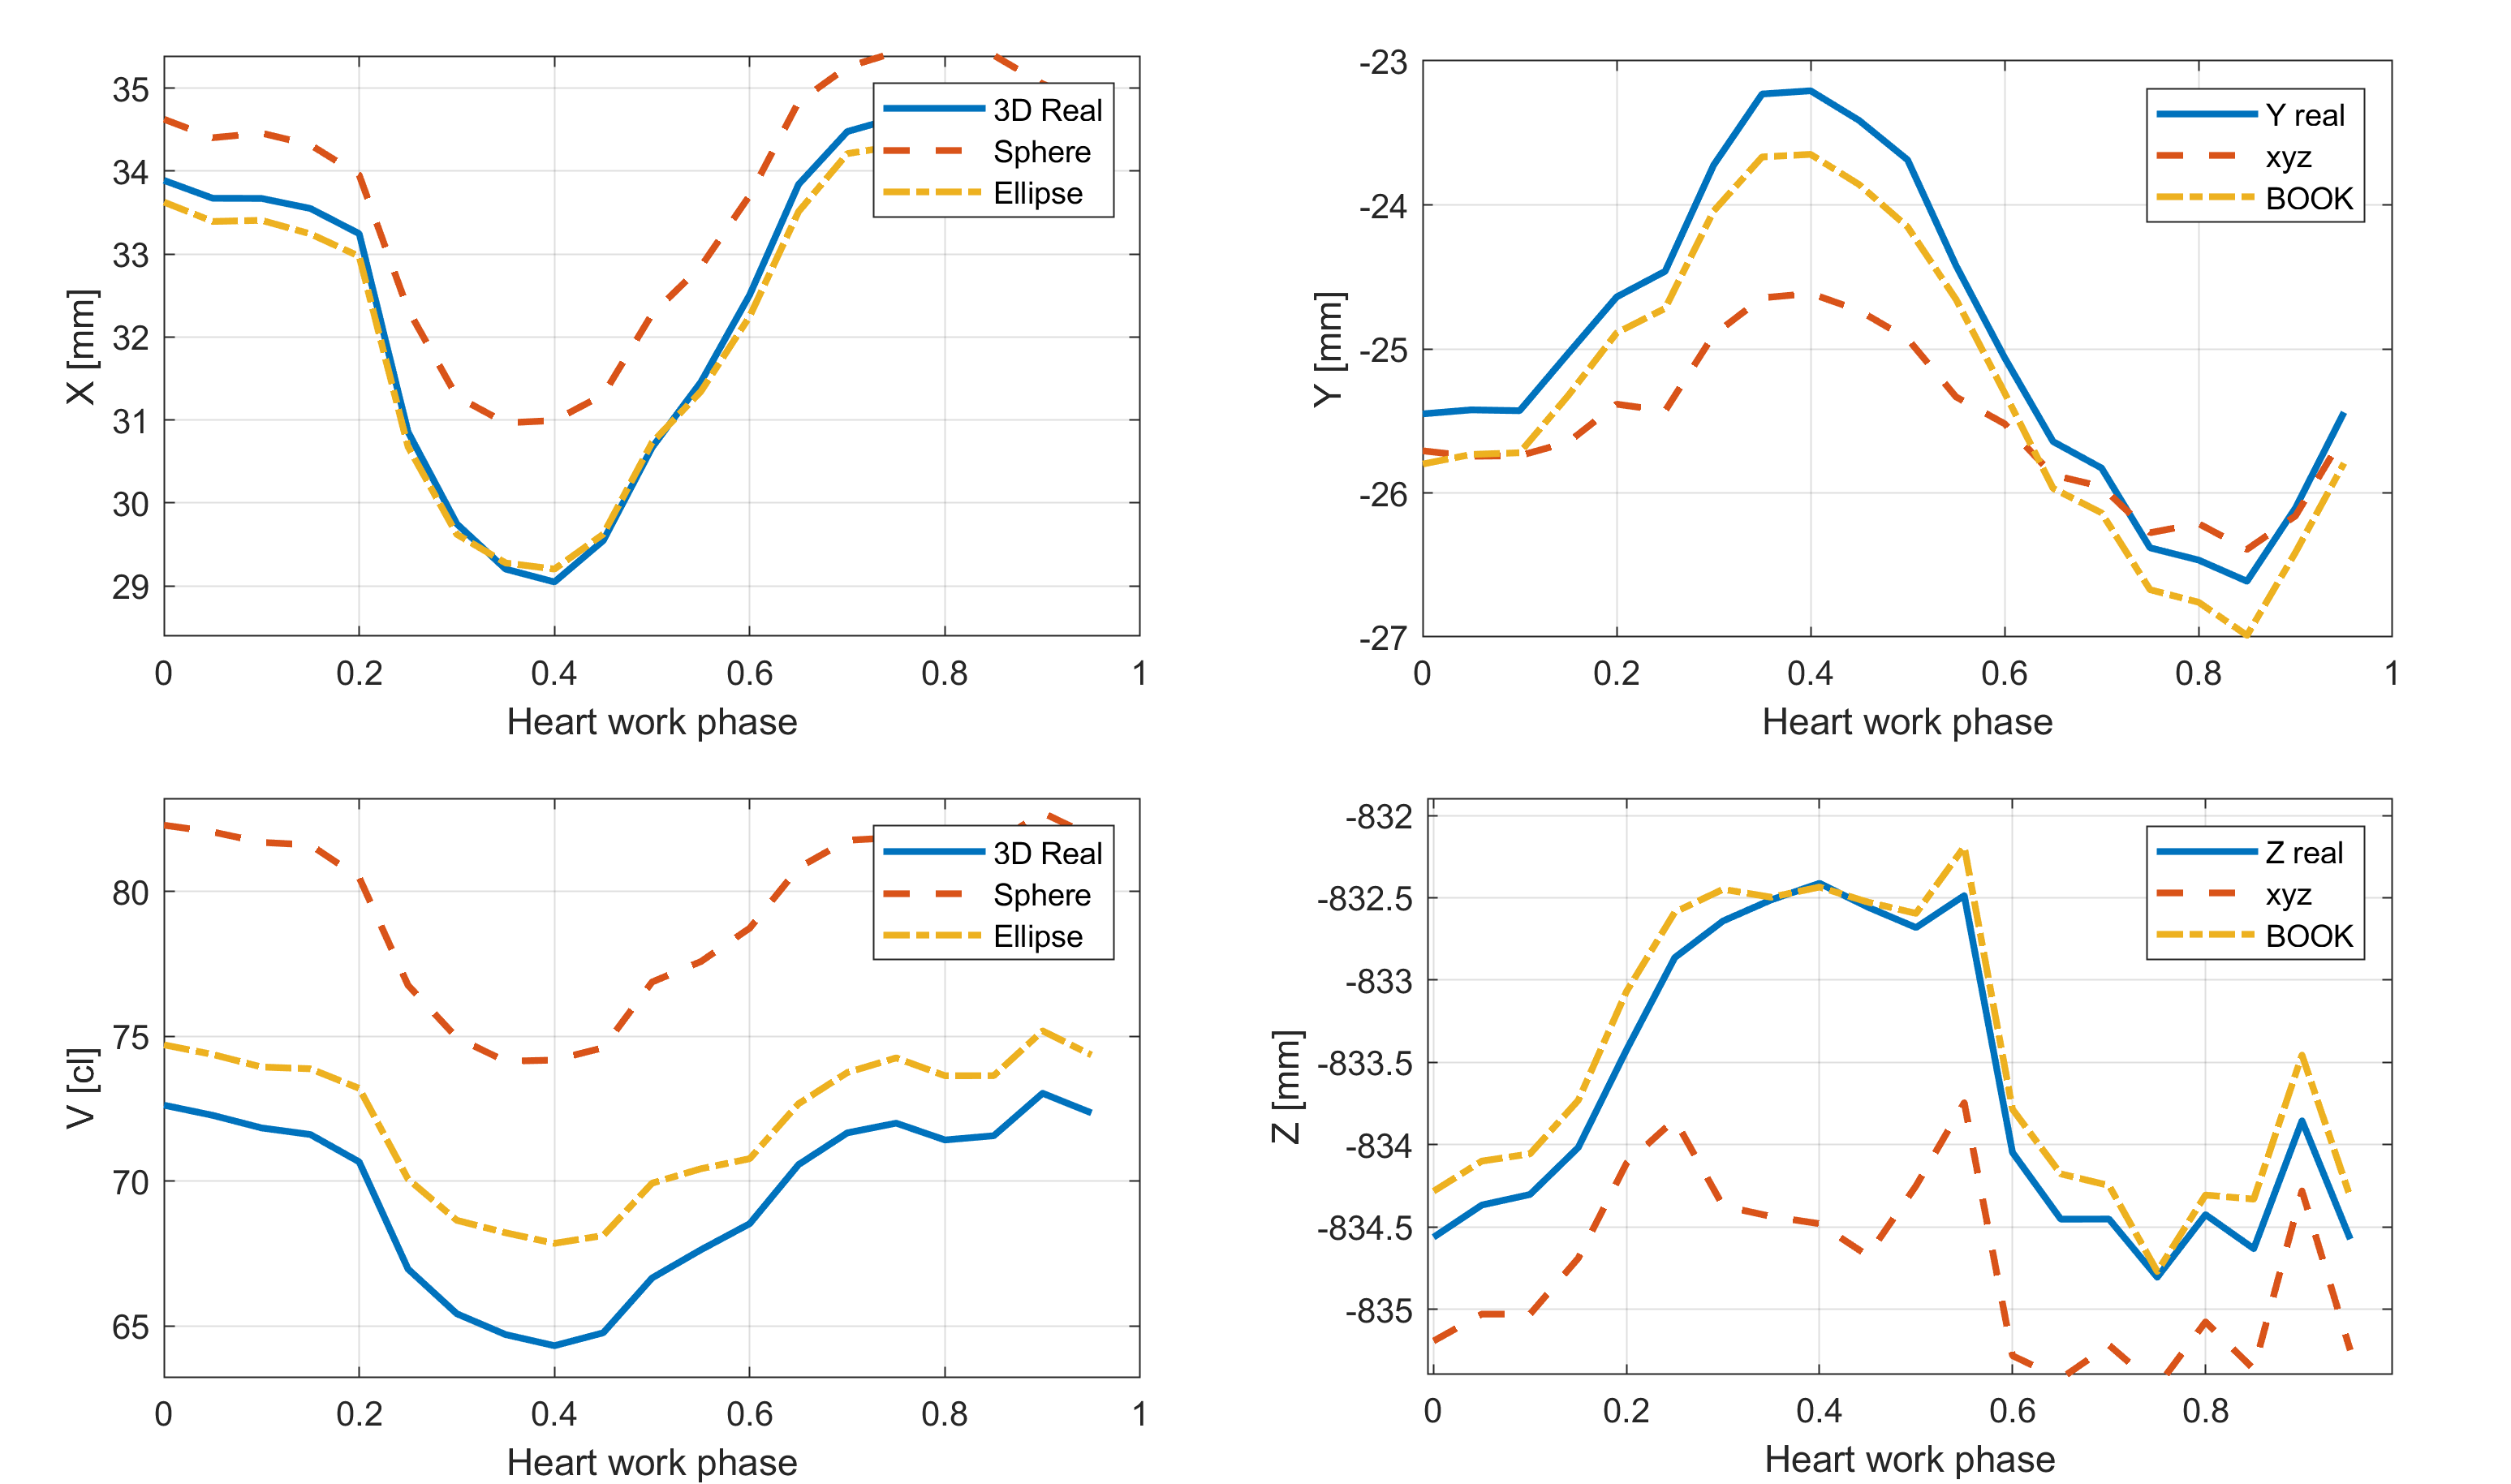
\includegraphics[width=\linewidth]{fig/1_4}}
    \caption{Изменение в ходе сердечного цикла координат центра масс (X, Y, Z) и объема исходной 3D модели, сферы и эллипсоида}
    \label{fig:rxyz}
\end{figure}

\section{Results}

Зависимости изменения объема и координат центра масс исходной 3D модели и аппроксимирующей сферы и эллипсоида представлены на Рис.~\ref{fig:rxyz},
где на временной шкале сердечный цикл от R-зубца до R-зубца.
% по оси абсцисс

Результаты моделирования изменения импеданса в ходе сердечного цикла представлены на Рис.~\ref{real},Рис.~\ref{fig:sphere},Рис.~\ref{fig:ellipse}.
Для каждой модели представлены зависимости для электродной системы расположенной вдоль анатомической оси сердца и перпендикулярно ей.
На этих графиках так же рассматривается сердечный цикл от R-зубца до R-зубца.

\begin{figure}[tbph]
    \centering
    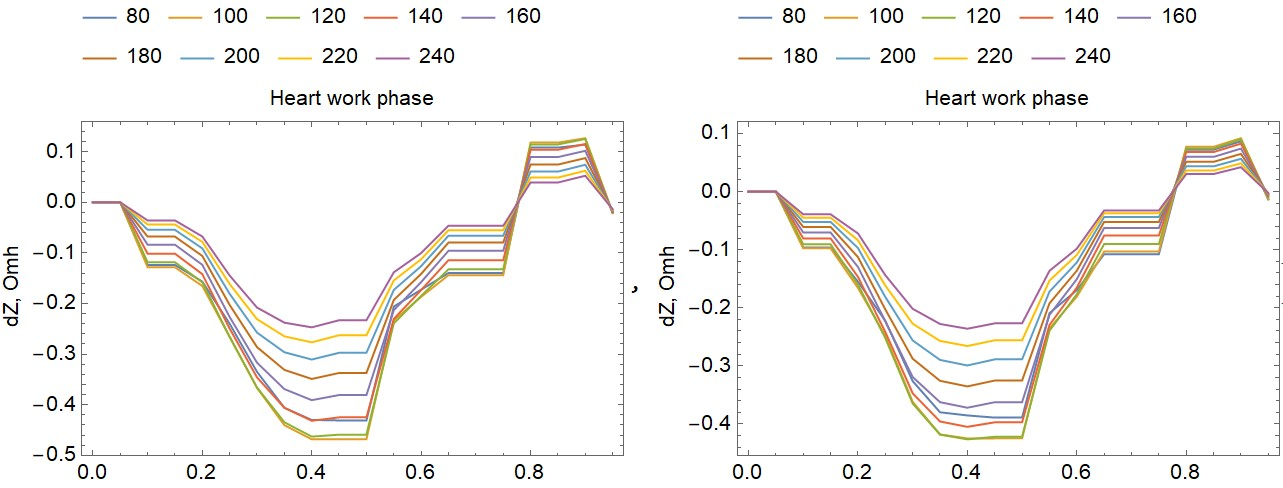
\includegraphics[width=\linewidth]{fig/real}
    \caption{Зависимость изменения импеданса в ходе сердечного цикла для исходной 3D модели (расположение электродной системы вдоль оси сердца - слева,перпендикулярно оси сердца - справа)}
    \label{real}
\end{figure}

\begin{figure}[tbph]
    \centering
    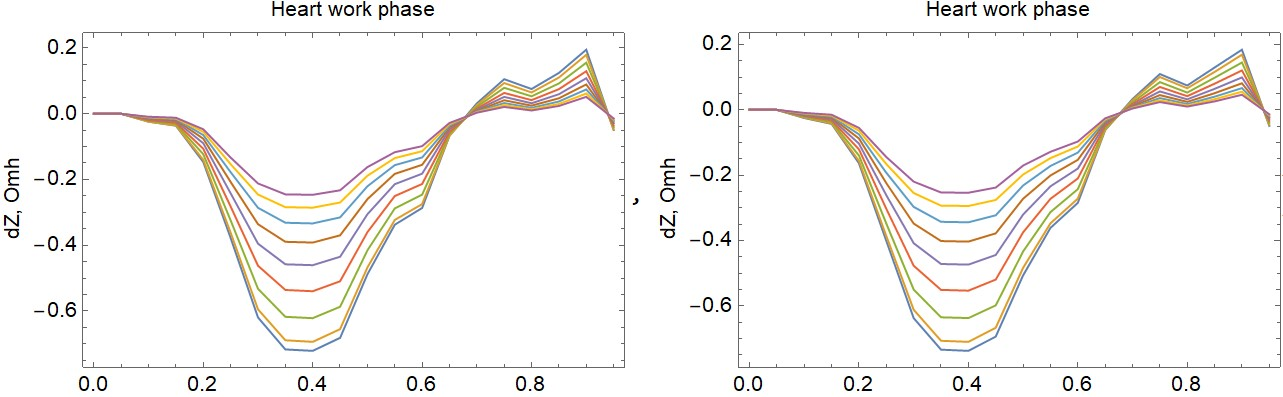
\includegraphics[width=\linewidth]{fig/sphere}
    \caption{Зависимость изменения импеданса в ходе сердечного цикла для сферической модели (расположение электродной системы вдоль оси сердца - слева,перпендикулярно оси сердца - справа)}
    \label{fig:sphere}
\end{figure}

\begin{figure}[tbph]
    \centering
    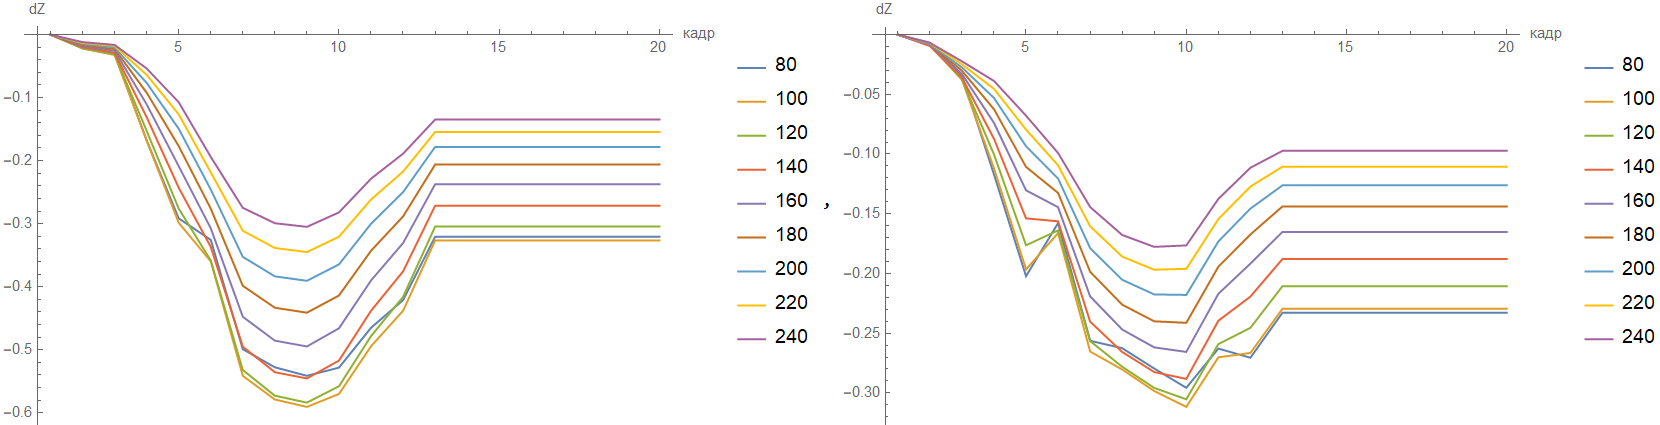
\includegraphics[width=\linewidth]{ellipse}
    \caption{Зависимость изменения импеданса в ходе сердечного цикла для эллиптической модели (расположение электродной системы вдоль оси сердца - слева,перпендикулярно оси сердца - справа)}
    \label{fig:ellipse}
\end{figure}



\section{Discussion}

При сравнении движения центра масс исходной 3D модели и аппроксимирующей сферы и эллипсоида из Рис.\ref{fig:rxyz} видно,
что центр масс эллипсоида движется в соответствии с центром масс 3D модели.
Движение сферы качественно соответствует движению 3D модели, но количественно отличается - менее амплитудное.
Объем эллипсоида отличается в среднем на 3-5\% в ходе сердечного цикла, для сферы разница достигает 12-15\%.
Это может оказать влияние и внести дополнительную погрешность при оценке гемодинамических характеристик на основе геометрической модели сферы.

Формы сигналов электроримпедансного моделирования для сферы и эллипсоида качественно соответсвуют форме сигнала для исходной 3D модели, но значительно отличаются по амплитудным характеристикам.
Для численной оценки полученных результатов моделирования сравнивалось значение изменения импеданса в ходе систолы желудочков $\Delta Z$.
То есть разности значений  на Рис.\ref{real}  в моменты времени соответствующие 0\% и 40\% кардиоцикла (начало и окончание систолы желудочков).
При малых значениях электродных систем (80-120 мм) $\Delta Z$ для 3D модели отличается на \%  от $\Delta Z$ для сферы и на \% от $\Delta Z$ для эллипсоида.
При больших значениях электродных систем (200-240 мм) $\Delta Z$ для 3D модели отличается на \%  от $\Delta Z$ для сферы и на \% от $\Delta Z$ для эллипсоида.
%todo заполнить проценты

\section{Conclusion}

Проведенные исследования показали, что для данного добровольца эллиптическая геометрическая модель крови сердца аппроксимирует реальную 3D геометрию сердца с погрешностью 3-5\% и является предпочтительной, при оценке гемодинамических параметров.
При этом электроимпедансное моделирование показало, что при использовании электродных систем размером 80--120 мм предпочтительно использовать эллиптическую геометрическую модель, а при использовании больших электродных систем 200--240 мм предпочтительно использовать сферическую геометрическую модель.
Так как для прекардиального продольно-поперечного картирования, как правило, используются электродные системы с размерами свыше 180 мм, то необходимо использовать сферическую математическую модель.

Указанные выводы верны для данного добровольца. На данный момент проводятся исследования еще для трех здоровых добровольцев, чтобы оценить полученные выводы.
%An excellent style manual for science writers is \cite{b7}.

\begin{thebibliography}{00}
\bibitem{b1} G. Eason, B. Noble, and I. N. Sneddon, ``On certain integrals of Lipschitz-Hankel type involving products of Bessel functions,'' Phil. Trans. Roy. Soc. London, vol. A247, pp. 529--551, April 1955.
\bibitem{b2} J. Clerk Maxwell, A Treatise on Electricity and Magnetism, 3rd ed., vol. 2. Oxford: Clarendon, 1892, pp.68--73.
\bibitem{b3} I. S. Jacobs and C. P. Bean, ``Fine particles, thin films and exchange anisotropy,'' in Magnetism, vol. III, G. T. Rado and H. Suhl, Eds. New York: Academic, 1963, pp. 271--350.
\bibitem{b4} K. Elissa, ``Title of paper if known,'' unpublished.
\bibitem{b5} R. Nicole, ``Title of paper with only first word capitalized,'' J. Name Stand. Abbrev., in press.
\bibitem{b6} Y. Yorozu, M. Hirano, K. Oka, and Y. Tagawa, ``Electron spectroscopy studies on magneto-optical media and plastic substrate interface,'' IEEE Transl. J. Magn. Japan, vol. 2, pp. 740--741, August 1987 [Digests 9th Annual Conf. Magnetics Japan, p. 301, 1982].
\bibitem{b7} M. Young, The Technical Writer's Handbook. Mill Valley, CA: University Science, 1989.
\end{thebibliography}
\vspace{12pt}
%\color{red}
%IEEE conference templates contain guidance text for composing and formatting conference papers. Please ensure that all template text is removed from your conference paper prior to submission to the conference. Failure to remove the template text from your paper may result in your paper not being published.

\end{document}
